%%%%%%%%%%%%%%%%%%%%%%%%%%%%%%%%%%%%%%%%%
% Jacobs Landscape Poster
% LaTeX Template
% Version 1.1 (14/06/14)
%
% Created by:
% Computational Physics and Biophysics Group, Jacobs University
% https://teamwork.jacobs-university.de:8443/confluence/display/CoPandBiG/LaTeX+Poster
% 
% Further modified by:
% Nathaniel Johnston (nathaniel@njohnston.ca)
%
% This template has been downloaded from:
% http://www.LaTeXTemplates.com
%
% License:
% CC BY-NC-SA 3.0 (http://creativecommons.org/licenses/by-nc-sa/3.0/)
%
%%%%%%%%%%%%%%%%%%%%%%%%%%%%%%%%%%%%%%%%%

%----------------------------------------------------------------------------------------
%	PACKAGES AND OTHER DOCUMENT CONFIGURATIONS
%----------------------------------------------------------------------------------------

\documentclass[final]{beamer}

\usepackage[scale=1.24]{beamerposter}

\usetheme{confposter}

\setbeamercolor{block title}{fg=dblue,bg=white}
\setbeamercolor{block body}{fg=black,bg=white}
\setbeamercolor{block alerted title}{fg=white,bg=dblue!70}
\setbeamercolor{block alerted body}{fg=black,bg=dblue!10}
\setbeamercolor{item}{fg=nblue}
\setbeamercolor{item projected}{fg=white,bg=nblue}

\newlength{\sepwid}
\newlength{\onecolwid}
\newlength{\twocolwid}
\newlength{\threecolwid}
\setlength{\paperwidth}{46.8in} % A0 width: 46.8in
\setlength{\paperheight}{33.1in} % A0 height: 33.1in
\setlength{\sepwid}{0.024\paperwidth} % Separation width (white space) between columns
\setlength{\onecolwid}{0.22\paperwidth} % Width of one column
\setlength{\twocolwid}{0.464\paperwidth} % Width of two columns
\setlength{\threecolwid}{0.708\paperwidth} % Width of three columns
\setlength{\topmargin}{-1.5in} % Reduce the top margin size

\usepackage{kmath}
% ------------------------ %
% 	  Packages		%
% ------------------------ %

\usepackage[utf8]{inputenc}
\usepackage[T1]{fontenc}
\usepackage{xcolor}
\usepackage{kmath}
\usepackage{xparse,pgffor,ifthen,xspace}
\usepackage{amsmath,amssymb,amsfonts,amsthm}
\usepackage{mathrsfs,mathtools,bbm}
\usepackage{booktabs,dcolumn,multirow,stmaryrd}
\newcolumntype{d}{D{.}{.}{3.2}}
\newcolumntype{e}{D{.}{.}{1.2}}
\usepackage{pgfplots,forest}
\pgfplotsset{compat=newest}
\usepackage[ruled,linesnumbered]{algorithm2e}
\usepackage{cleveref,csquotes,comment,lipsum,todonotes,soul}
\usepackage{glossaries,url,subcaption}
% ------------------------ %
% 	  Shortcuts		  %
% ------------------------ %

% Lowercase styles
\foreach \x in {a,...,z}{%
	\expandafter\xdef\csname \x\endcsname{\noexpand\ensuremath{\noexpand\mathbf{\x}}}
}
\foreach \x in {a,...,z}{%
	\expandafter\xdef\csname \x rm\endcsname{\noexpand\ensuremath{\noexpand\mathrm{\x}}}
}

% Uppercase styles
\foreach \x in {A,...,Z}{%
	\expandafter\xdef\csname \x\endcsname{\noexpand\ensuremath{\noexpand\mathbf{\x}}}
}
\foreach \x in {A,...,Z}{%
	\expandafter\xdef\csname \x rm\endcsname{\noexpand\ensuremath{\noexpand\mathrm{\x}}}
}
\foreach \x in {A,...,Z}{%
	\expandafter\xdef\csname \x bb\endcsname{\noexpand\ensuremath{\noexpand\mathbb{\x}}}
}
\foreach \x in {A,...,Z}{%
	\expandafter\xdef\csname \x c\endcsname{\noexpand\ensuremath{\noexpand\mathcal{\x}}}
}

% Figures styles
\def\0{{\mathbf 0}}
\def\1{{\mathbf 1}}

% Miscellaneous
\def\ie{\emph{i.e.,}\xspace}
\def\eg{\emph{e.g.,}\xspace}
\def\etal{\emph{et al.}\xspace}
\def\resp{resp.\xspace}
\def\iif{iff.\xspace}
%\def\st{\ensuremath{\mathrm{st.}}\xspace}

% Notes
\def\addNote#1{{\noindent\color{blue}{[Note : #1]}}}
\def\toDo#1{{\noindent\color{red}{[Todo : #1]}}}
\def\addCite{{\noindent\color{orange}{[Cite]}}}
% ------------------------ %
% 			Macros		   %
% ------------------------ %

% Fonts
\newcommand{\fontset}[1]{\mathcal{#1}}
\newcommand{\fontnode}[1]{\text{\scshape#1}}
\newcommand{\fontoptpb}[1]{#1}

% Data
\newcommand{\pdim}{n}
\newcommand{\ddim}{m}
\newcommand{\obs}{\y}
\newcommand{\dic}{\A}
\newcommand{\atom}{\a}
\newcommand{\reg}{\lambda}
\newcommand{\bigM}{M}
\newcommand{\pivot}[2]{\boldsymbol{\gamma}_{#1}^{#2}}

% Screening sets
% \newcommand{\nodeSymb}{\fontnode{n}}
\newcommand{\nodeSymb}{\nu}
\newcommand{\nodeSymbIter}[1]{\nodeSymb^{(#1)}}
\newcommand{\setnodesymb}{\fontset{S}}
\newcommand{\setzero}{\setnodesymb_0}
\newcommand{\setone}{\setnodesymb_1}
\newcommand{\setnone}{\bar{\setnodesymb}}

\newcommand{\nodePlusZero}[2]{#1\cup\{\pve_{#2}=0\}}
\newcommand{\nodePlusOne}[2]{#1\cup\{\pve_{#2}\neq0\}}

% Superscripts and subscripts
\newcommand{\subzero}[1]{#1_{\setzero}}
\newcommand{\subone}[1]{#1_{\setone}}
\newcommand{\subnone}[1]{#1_{\setnone}}
\newcommand{\node}[1]{#1^{\nodeSymb}}

% Upper/Lower bounds on optimal values
\newcommand{\UB}[1]{#1_u}
\newcommand{\LB}[1]{#1_{l}}

% Problems
\newcommand{\primalletter}{\fontoptpb{P}}
\newcommand{\dualletter}{\fontoptpb{D}}
\newcommand{\mpb}{\primalletter}
\newcommand{\spb}{\primalletter}
\newcommand{\hpb}{\UB{\primalletter}}
\newcommand{\rpb}{\LB{\primalletter}}
\newcommand{\dpb}{\dualletter}

% Objective values
\newcommand{\pobj}{p}
\newcommand{\optobj}{\opt{\pobj}}
\newcommand{\sobj}{\pobj}
\newcommand{\hobj}{\UB{\sobj}}
\newcommand{\robj}{\LB{\sobj}}
\newcommand{\dobj}{d_l}

% Objective functions
\newcommand{\pfunc}{\Prm}
\newcommand{\hfunc}{\UB{\pfunc}}
\newcommand{\rfunc}{\LB{\pfunc}}
\newcommand{\dfunc}{\Drm_{l}}
		
% Variables
\newcommand{\pve}{x}
\newcommand{\bve}{z}
\newcommand{\dve}{u}
\newcommand{\pv}{\mathbf{\pve}}
\newcommand{\pvrelax}{\mathbf{\pve}_l}
\newcommand{\bv}{\mathbf{\bve}}
%\newcommand{\dv}{\mathbf{\dve}_l}
\newcommand{\dv}{\mathbf{\dve}}
\newcommand{\dvopt}{\dv^\star_l}

\newcommand{\idxentrynode}{i}
\newcommand{\idxscreen}{\ell}

% Operators
\newcommand{\argmin}{\mathrm{argmin}}
\newcommand{\argmax}{\mathrm{argmax}}
\newcommand{\conj}[1]{#1^*}
\newcommand{\card}[1]{|#1|}
\newcommand{\grad}{\nabla}
\newcommand{\Icvx}{\eta}
\newcommand{\intervint}[2]{\llbracket#1,#2\rrbracket}
\newcommand{\norm}[2]{\|#1\|_#2}
\newcommand{\opt}[1]{#1^{\star}}
\newcommand{\scalprod}[2]{\langle{#1,#2}\rangle}
\newcommand{\sign}[1]{\mathrm{sign}({#1})}
\newcommand{\relu}[1]{[#1]_+}

\DeclarePairedDelimiter\ceil{\lceil}{\rceil}
\DeclarePairedDelimiter\floor{\lfloor}{\rfloor}

\usepackage[pscoord]{eso-pic}
\newcommand{\placetextbox}[3]{
  \setbox0=\hbox{#3}
  \AddToShipoutPictureFG*{
    \put(\LenToUnit{#1\paperwidth},\LenToUnit{#2\paperheight}){\vtop{{\null}\makebox[0pt][c]{#3}}}
  }
}

\newcommand{\emphone}[1]{\textit{\color{norange}#1}}

\newacronym{bnb}{BnB}{Branch-and-Bound}
\newacronym{mip}{MIP}{Mixed-Integer Program}
\newcommand{\METHOD}{NODE-SCREENING\xspace}
\newcommand{\Method}{Node-screening\xspace}
\newcommand{\method}{node-screening\xspace}
\newcommand{\sparsitylevel}{k}
\newcommand{\sparsevector}{\pv^0}
\newcommand{\CPLEX}{\texttt{Direct}}
\newcommand{\BNB}{\texttt{BnB}}
\newcommand{\BNBscr}{\texttt{BnB+scr}}

%----------------------------------------------------------------------------------------
%	TITLE SECTION 
%----------------------------------------------------------------------------------------

\title{Node-screening tests for the $\ell_0$-penalized least-squares problem}

\author{Théo Guyard${}^{\star}$, Cédric Herzet${}^{\dagger}$, Clément Elvira${}^{\ddagger}$}

\institute{${}^{\star}$Applied Mathematics Department, INSA Rennes, France | ${}^{\dagger}$SIMSMART team, INRIA Rennes-Bretagne Atlantique, France | ${}^{\ddagger}$SCEE team, CentraleSupelec Rennes, France}

%----------------------------------------------------------------------------------------

\begin{document}

\placetextbox{0.955}{0.995}{\fbox{Paper ID : 2482}}

\addtobeamertemplate{block end}{}{\vspace*{2ex}}
\addtobeamertemplate{block alerted end}{}{\vspace*{2ex}}

\setlength{\belowcaptionskip}{2ex}
\setlength\belowdisplayshortskip{2ex}

\begin{frame}[t]
\begin{columns}[t]

\begin{column}{\sepwid}\end{column}

\begin{column}{\onecolwid}

    \begin{alertblock}{Objectives}
        Reduce the optimization time of a \gls{bnb} solving the $\ell_0$-penalized least-squares problem by detecting nodes of the search tree that cannot yield a global optimizer.
    \end{alertblock}

    \begin{block}{Introduction}
        \begin{itemize}
            \item \hspace*{0.1em} Sparse decomposition aims at finding some approximation of a vector $\obs$ as the linear combination of a few columns of a dictionary $\dic$. The $\ell_0$-penalized least-squares problem is one way to achieve this :
        \end{itemize}
        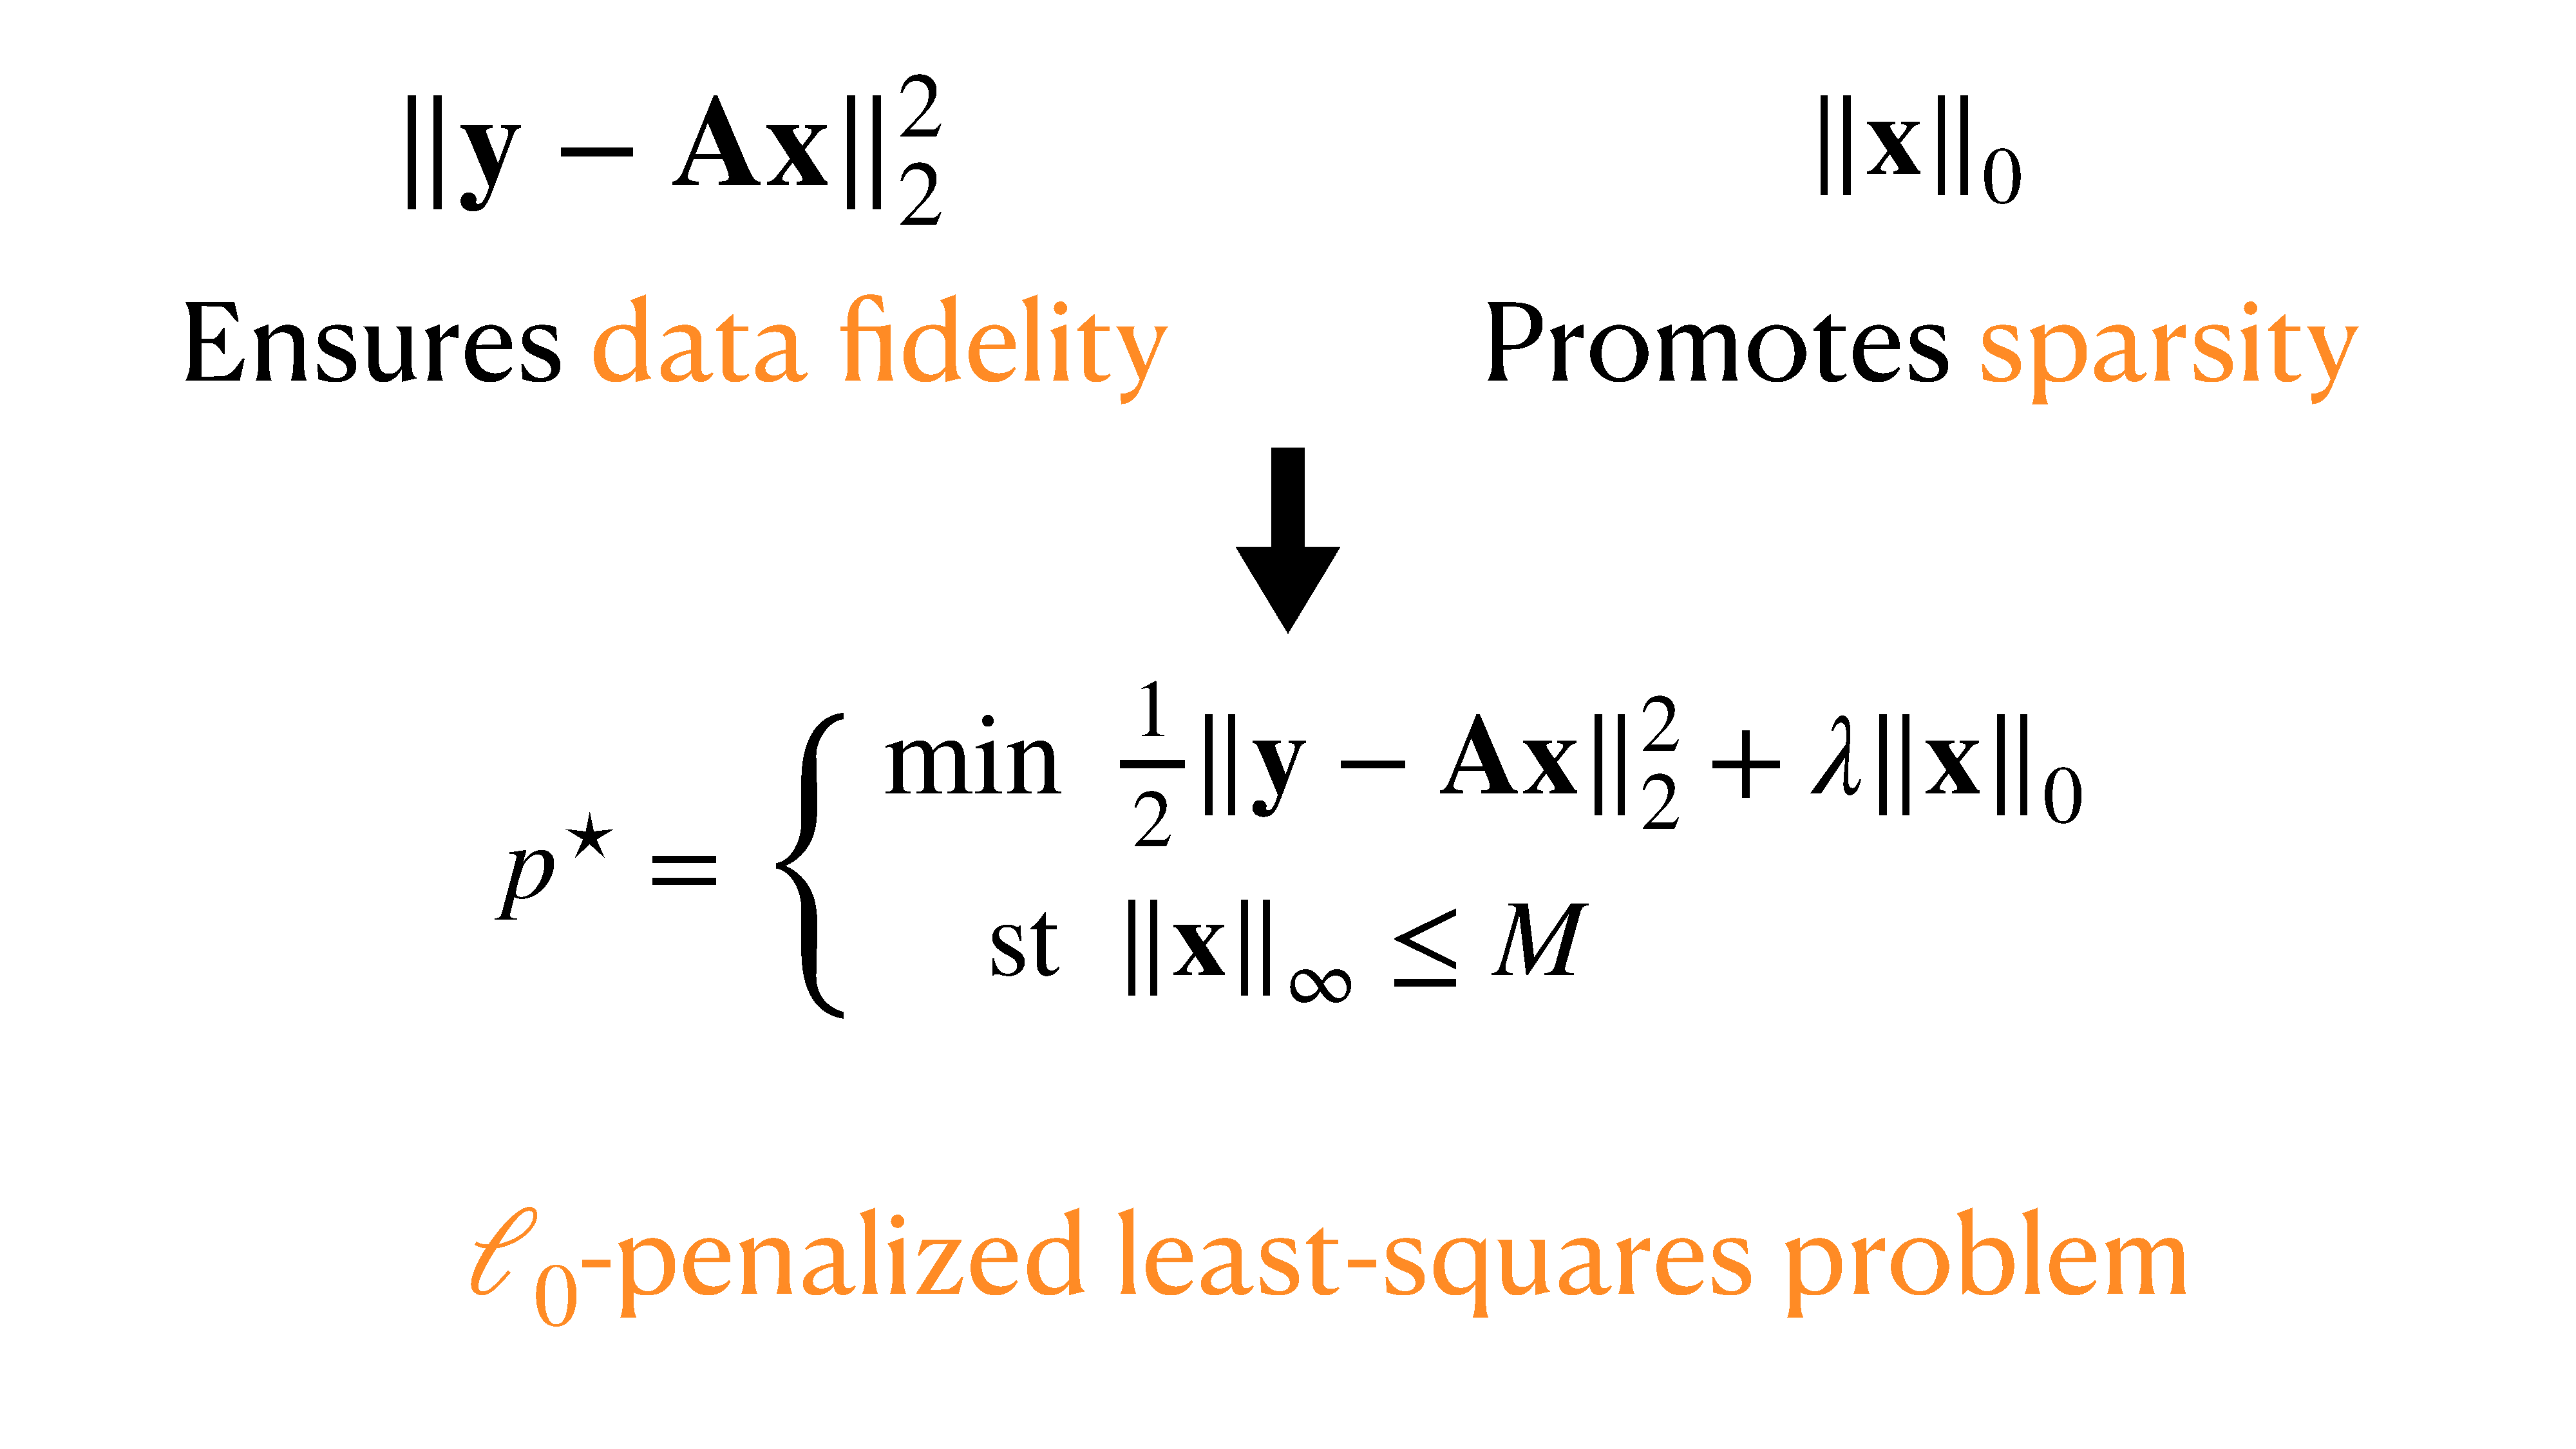
\includegraphics[width=\linewidth]{imgs/problem.pdf}
        \vspace*{-2em}
        \begin{itemize}
            \item \hspace*{0.1em} Highlights :
            \begin{itemize}
                \normalsize \item[-] \hspace*{0.1em} NP-hard problem
                \item[-] \hspace*{0.1em} \gls{mip} reformulation thanks to the Big-M constraint
                \item[-] \hspace*{0.1em} Addressable with \gls{bnb} algorithms  
            \end{itemize}
        \end{itemize}

        \begin{itemize}
            \item \hspace*{0.1em} Recent advances by Atamturk \textit{et. al.} :
            \begin{itemize}
                \normalsize \item[-] \hspace*{0.1em} \emphone{Screening tests} to detect zero and non-zero element of the solution
                \item[-] \hspace*{0.1em} This allows a dimensionality reduction in \emphone{pre-processing}
            \end{itemize}
        \end{itemize}

        \begin{itemize}
            \item \hspace*{0.1em} Our contributions :
            \begin{itemize}
                \normalsize \item[-] \hspace*{0.1em} \emphone{Node-screening tests} to detect \emphone{combinations} of zero and non-zero elements that cannot yield an optimal solution.
                \item[-] \hspace*{0.1em} This allows a dimensionality reduction at \emphone{any step of the optimization process}.
            \end{itemize}
        \end{itemize}
    \end{block}
\end{column}

\begin{column}{\sepwid}\end{column}

\begin{column}{\twocolwid}    
    \begin{columns}[t,totalwidth=\twocolwid]
        \begin{column}{\onecolwid}\vspace{-.6in} 
            
            \begin{block}{\gls{bnb} procedures}
                \begin{itemize}
                    \item \hspace*{0.1em} Generic procedure :
                \end{itemize}
                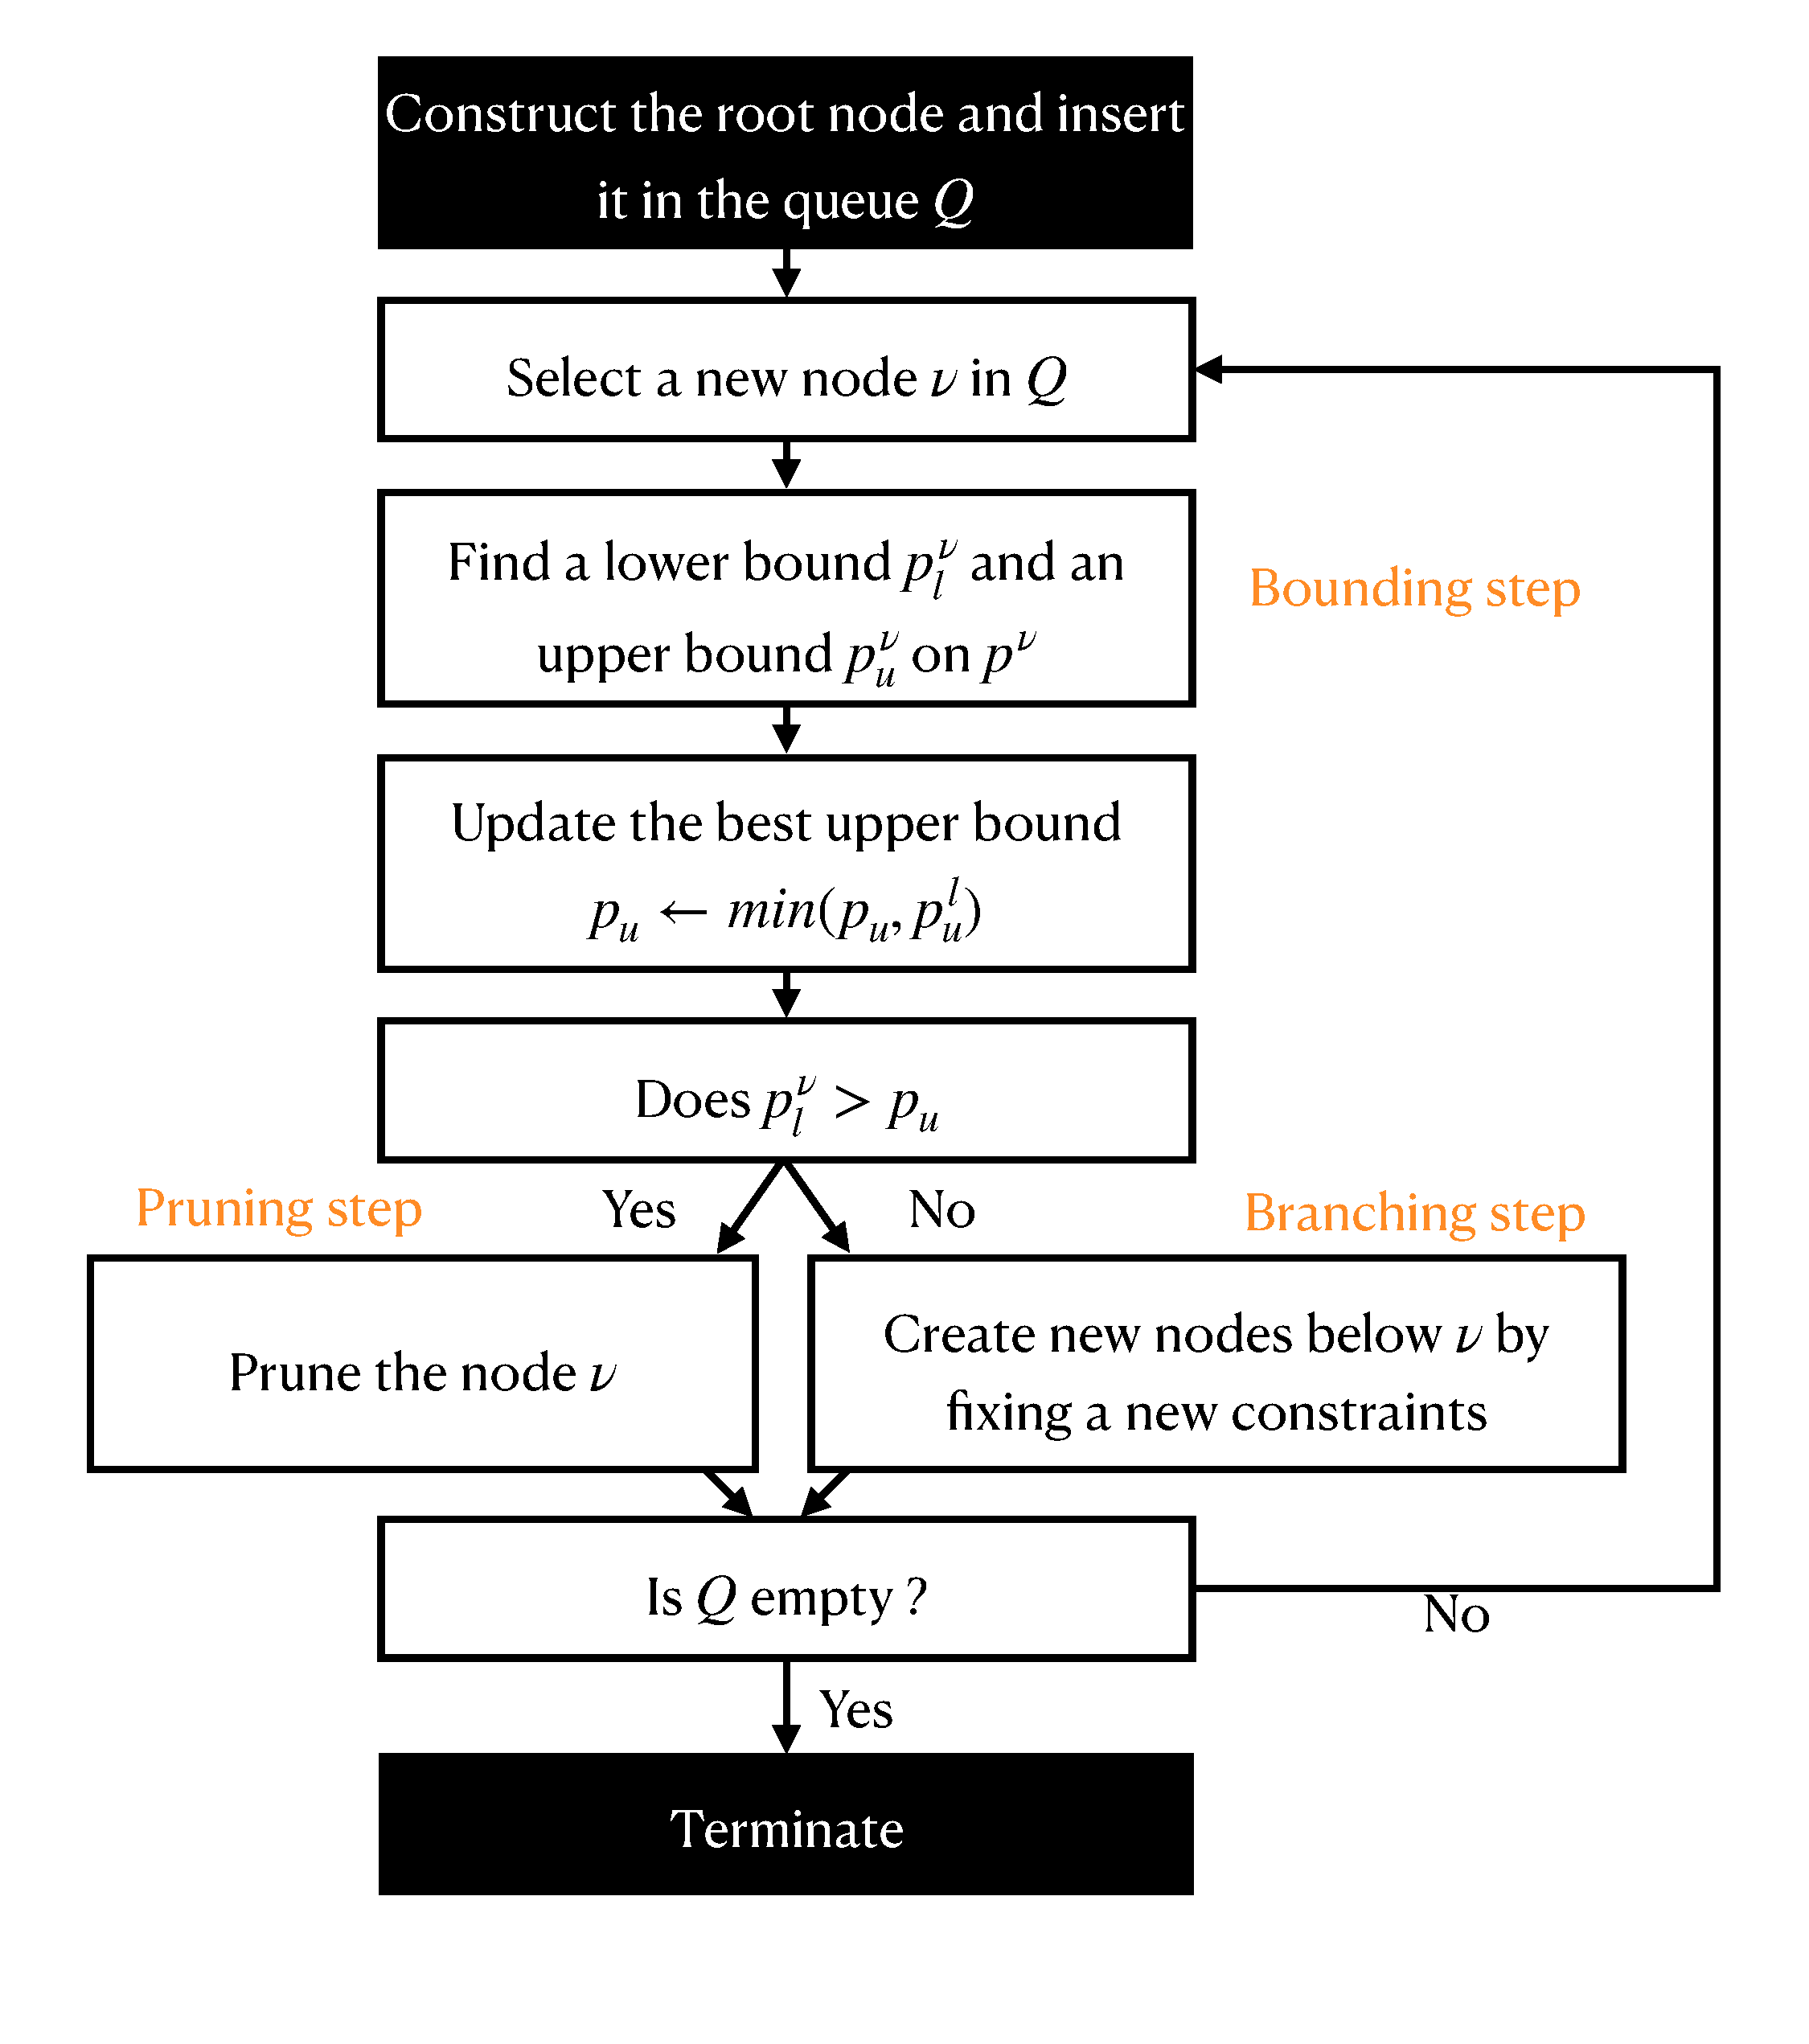
\includegraphics[width=\linewidth]{imgs/bnb.pdf}
                \vspace*{-3em} 
                \begin{itemize}
                    \item \hspace*{0.1em} Particularized to our problem :
                    \begin{itemize}
                        \normalsize \item[-] \hspace*{0.1em} Binary decision tree where new decision concerning the \emphone{nullity of a coefficient} is taken at each node
                        \item[-] \hspace*{0.1em} Each node is defined by $(\setzero,\setone,\setnone)$ where \(\setzero\) and \(\setone\) contain the indices which are forced to be \emphone{zero} and \emphone{non-zero} and where \(\setnone\) gathers all the \emphone{unfixed} indices.
                    \end{itemize}
                \end{itemize}
                \begin{itemize}
                    \item \hspace*{0.1em} What impacts the efficiency of the algorithm :
                    \begin{itemize}
                        \normalsize \item[-] \hspace*{0.1em} Number of nodes processed
                        \item[-] \hspace*{0.1em} Ability to process nodes quickly
                    \end{itemize}
                \end{itemize}
            \end{block}
        \end{column}

        \begin{column}{\onecolwid}\vspace{-.6in}
            \begin{block}{Node-screening tests}
                \begin{itemize}
                    \item \hspace*{0.1em} Underlying idea :
                    \begin{itemize}
                        \normalsize \item[i)] \hspace*{0.1em} We are at a given node $\nu$
                        \item[ii)] \hspace*{0.1em} We select an unfixed index $i$
                        \item[iii)] \hspace*{0.1em} We compute a lower bound $d_l^{\nu \cup \{i\}}$ on $p_l^{\nu \cup \{i\}}$ at a \emphone{very low computational cost}
                        \item[iv)] \hspace*{0.1em} If $d_l^{\nu \cup \{i\}} > p_u$, then the node $\nu \cup \{i\}$ needs not be explored 
                    \end{itemize}
                \end{itemize}
                But ... It is like the pruning step isn't it ?
                \begin{itemize}
                    \item \hspace*{0.1em} Differences with the pruning step :
                    \begin{itemize}
                        \normalsize \item[-] \hspace*{0.1em} We can test \emphone{any} unfixed index
                        \item[-] \hspace*{0.1em} Node-screening tests \emphone{do not bring any computational overhead}
                        \item[-] \hspace*{0.1em} They allow to fix \emphone{multiple variables simultaneously}
                    \end{itemize}
                \end{itemize}
            \end{block}
            \begin{alertblock}{Main ingredients}
                \begin{itemize}
                    \item \hspace*{0.1em} In the \gls{bnb}, $p_l^{\nu}$ is obtained by solving the \emphone{convex relaxation} of the initial problem with the current node constraints
                    \item \hspace*{0.1em} We construct the \emphone{dual} of this relaxation
                    \item \hspace*{0.1em} Duals have a very similar expression between consecutive nodes
                    \item \hspace*{0.1em} This allows compute the lower bound $d_l^{\nu \cup \{i\}}$ with no additional cost for several $i$
                    \item \hspace*{0.1em} And therefore to prune \emphone{multiple nodes} simultaneously !
                \end{itemize}
            \end{alertblock}
        \end{column}
    \end{columns}

    \begin{figure}
        \begin{subfigure}[b]{0.49\textwidth}
            \centering
            \forestset{
    node/.style = {
        draw, 
        circle,
        thick,
        align = center,
        font = \scriptsize,
        top color = white,
        bottom color = blue!25,
    },
    branch label/.style={
        edge label = {
            node[midway,fill=white,font=\scriptsize,draw=black,text height=0.5em,scale=0.9]{#1}
        }
    },
    bnb/.style={
        branch label,
        for tree = {
            node,
            s sep'+=45mm,
            l sep'+=0mm,
            edge={->},
            edge+={thick},
        },
        before typesetting nodes={
            for tree={
                split option={content}{:}{content,branch label},
            },
        },
        where n children=0{
            tikz+={
                \draw [thick,dashed,->]  ([yshift=0pt, xshift=0pt].south east) -- ([yshift=-5pt, xshift=5pt].south east);
                \draw [thick,dashed,->]  ([yshift=0pt, xshift=0pt].south west) -- ([yshift=-5pt, xshift=-5pt].south west);
            }
        }{},
    },
}
\begin{forest}
    bnb,
    [
        \(\nodeSymbIter{0}\)
            [\(\nodeSymbIter{1}\):\({\pve_{\idxentrynode_1}=0}\)
            [\(\nodeSymbIter{3}\):\({\pve_{\idxentrynode_2}=0}\)]
            [\(\nodeSymbIter{4}\):\({\pve_{\idxentrynode_2}\neq0}\)]
    ][
        \(\nodeSymbIter{2}\):\({\pve_{\idxentrynode_1}\neq0}\),
            [\(\nodeSymbIter{5}\):\({\pve_{\idxentrynode_2}=0}\)]
            [\(\nodeSymbIter{6}\):\({\pve_{\idxentrynode_2}\neq0}\)]
    ]
    ]
\end{forest}
        \end{subfigure}
        \hfill
        \begin{subfigure}[b]{0.49\textwidth}
            \centering
            \forestset{
    node/.style = {
        draw, 
        circle,
        thick,
        align = center,
        font = \scriptsize,
        top color = white,
        bottom color = blue!25,
    },
    branch label/.style={
        edge label = {
            node[midway,fill=white,font=\scriptsize,draw=black,text height=0.5em,scale=0.9]{#1}
        }
    },
    bnb/.style={
        branch label,
        for tree = {
            node,
            s sep'+=45mm,
            l sep'+=0mm,
            edge={->, thick, draw opacity=0.2, text opacity = 0.3},
            opacity = 0.25,
            text opacity = 0.25,
        },
        before typesetting nodes={
            for tree={
                split option={content}{:}{content,branch label},
            },
        },
        where n children=0{
            tikz+={
                \draw [thick,dashed,->,opacity=0.25] ([yshift=0pt, xshift=0pt].south east) -- ([yshift=-5pt, xshift=5pt].south east);
                \draw [thick,dashed,->,opacity=0.25]  ([yshift=0pt, xshift=0pt].south west) -- ([yshift=-5pt, xshift=-5pt].south west);
            }
        }{},
    },
}
\begin{forest}
    bnb,
    [\(\nodeSymbIter{0}\),name=root,opacity=1,text opacity=1
        [\(\nodeSymbIter{1}\):\({\pve_{\idxentrynode_1}=0}\)
            [\(\nodeSymbIter{3}\):\({\pve_{\idxentrynode_2}=0}\),name=S3,opacity=1,text opacity=1] {
                \draw [thick,dashed,->] ([yshift=0pt, xshift=0pt].south east) -- ([yshift=-5pt, xshift=5pt].south east);
                \draw [thick,dashed,->]  ([yshift=0pt, xshift=0pt].south west) -- ([yshift=-5pt, xshift=-5pt].south west);
                \draw[thick,->] (root.west) .. controls (-10,0) .. (S3.north);
                \node[draw,thick,top color = white,
                bottom color = orange!25,,font=\scriptsize,align=center] at (-10,-0.4) (scr) {\bf {\scriptsize \Method} \\ Fix \({\pve_{\idxentrynode_1}=0}\) \\ Fix \({\pve_{\idxentrynode_2}=0}\)};
            }
            [\(\nodeSymbIter{4}\):\({\pve_{\idxentrynode_2}\neq0}\)]
        ]
        [\(\nodeSymbIter{2}\):\({\pve_{\idxentrynode_1}\neq0}\),
            [\(\nodeSymbIter{5}\):\({\pve_{\idxentrynode_2}=0}\)]
            [\(\nodeSymbIter{6}\):\({\pve_{\idxentrynode_2}\neq0}\)]
        ]
    ]
\end{forest}
        \end{subfigure}
    \end{figure}
\end{column}

\begin{column}{\sepwid}\end{column}

\begin{column}{\onecolwid}
    \begin{block}{Numerical results}
        \begin{itemize}
            \item \hspace{0.1in} Data generation :
            \begin{itemize}
                \normalsize \item[1)] \hspace{0.1in} \normalsize Generate a random matrix $\dic \in \kR^{500\times1000}$ with a correlation $\rho$ between the columns
                \item[2)] \hspace{0.1in} \normalsize Generate a $k$-sparse vector $\pv^{\dagger} \in \kR^{\pdim}$
                \item[3)] \hspace{0.1in} \normalsize Set $\obs = \dic\pv^{\dagger} + \text{noise with 10dB SNR}$
                \item[4)] \hspace{0.1in} \normalsize Calibrate $\lambda$ and $M$ statistically to recover $\pv^{\dagger}$
            \end{itemize}
        \end{itemize}
        ~\\
        \begin{itemize}
            \item \hspace{0.1in} Concurrent methods :
            \begin{itemize}
                \normalsize \item[-] \hspace{0.1in} \normalsize Direct method using CPLEX
                \item[-] \hspace{0.1in} \normalsize Tailored \gls{bnb} algorithm from Mhenni \textit{et. al.} 
                \item[-] \hspace{0.1in} \normalsize Tailored \gls{bnb} algorithm with \emphone{node-screening}
            \end{itemize}
        \end{itemize}

        \vspace{0.5in}
        \setlength{\tabcolsep}{6pt}

\begin{table}[!ht]
	\small
	\centering
    \begin{tabular}{cc||c|c|c||c|c|c||c|c|c}
	\toprule
	& & \multicolumn{3}{c||}{\CPLEX{}} & \multicolumn{3}{c||}{\BNB{}} & \multicolumn{3}{c}{\BNBscr{}} \\
	$\rho$ & \(\sparsitylevel\) & \multicolumn{1}{c}{N} & \multicolumn{1}{c}{T} & \multicolumn{1}{c||}{F} & \multicolumn{1}{c}{N} & \multicolumn{1}{c}{T} & \multicolumn{1}{c||}{F} & \multicolumn{1}{c}{N} & \multicolumn{1}{c}{T} & \multicolumn{1}{c}{F} \\ \midrule\midrule
    & \(5\) & 96 & 25.9 & 0 & 70 & 1.5 & 0 & \textbf{56} & \textbf{0.7} & \textbf{0} \\
    & \(7\) & 292 & 60.8 & 0 & 180 & 5.1 & 0 & \textbf{152} & \textbf{3.0} & \textbf{0} \\ 
    \parbox[t]{8mm}{\multirow{-3}{*}{\rotatebox[origin=c]{90}{Low}}} & \(9\) & 781 & 102.6 & 10 & 483 & 15.6 & 0 & \textbf{412} & \textbf{9.8} & \textbf{0} \\ \midrule
	& \(5\) & 1,424 & 10.2 & 0 & 965 & 6.4 & 0 & \textbf{725} & \textbf{4.2} & \textbf{0} \\
    & \(7\) & 17,647 & 106.5 & 0 & 10,461 & 79.3 & 0 & \textbf{7,881} & \textbf{52.2} & \textbf{0} \\ 
    \parbox[t]{8mm}{\multirow{-3}{*}{\rotatebox[origin=c]{90}{High}}} & \(9\) & 80,694 & 353.4 & 50 & 47,828 & 346.4 & 48 & \textbf{41,166} & \textbf{267.0} & \textbf{40} \\ \bottomrule                      
    \end{tabular}
	\caption{
		\small
		\label{tab:figure}
		Number of nodes explored (N), solving time in sec (T) and number of instances not solved within $10^3$ sec (F).
	}
\end{table}


        \begin{itemize}
            \item \hspace{0.1in} Observations :
            \begin{itemize}
                \normalsize \item[-] \hspace*{0.1in}\BNBscr~outperforms the two other methods
                \item[-] \hspace*{0.1in} The reduction in the solution time is more important than the reduction in the number of nodes explored
                \item[-] \hspace*{0.1in} Double kiss-cool effect : the bounding step is performed all the faster as \emphone{many variables are fixed} by the node-screening tests
            \end{itemize}
        \end{itemize}
        \begin{alertblock}{Take home message}
            In a \gls{bnb} applied to a sparse problem, there is not always need to spend too much computation in the bounding process.
            Many nodes that can be \emphone{easily pruned} by performing \emphone{simpler and cheaper tests} like the node-screening one.
        \end{alertblock}
        % \textbf{Take home message :} In a \gls{bnb} applied to a sparse problem, there is not always need to spend too much computation in solving a relaxation as it is classically done
        % Many nodes that can be easily pruned by performing simple and cheap tests like the node-screening one that we propose.
    \end{block}
\end{column} 

\begin{column}{\sepwid}\end{column}

\end{columns}
\end{frame}

\end{document}
